\documentclass[a4paper, 12pt]{report}
\usepackage[T2A]{fontenc}
\usepackage[english, russian]{babel}
\usepackage{graphicx}
\graphicspath{{./images/}}
\usepackage[utf8]{inputenc}
\usepackage[backend=biber,bibencoding=utf8,sorting=nty,maxcitenames=2,style=numeric-comp]{biblatex}
\addbibresource{bibliography.bib}

\begin{document}
	\chapter{Обезьяны}
	\section{Кто такие обезьяны}
	
Обезья́ны — группа млекопитающих из отряда приматов. В биологической систематике название «обезьяны» может применяться по отношению ко всем представителям инфраотряда Simiiformes или подотряда Haplorhini[2][3][4] (оба таксона включают человека, который не является обезьяной в обиходном смысле слова; второй таксон, помимо представителей Simiiformes, включает также долгопятов).

Карл Линней включил в состав рода Simia[en] всех приматов, кроме лемуров, которых он объединил с шерстокрылами в род Lemur, а также людей, орангутанов и шимпанзе, которых он включил в состав рода Homo[5][6]. Во многих устаревших классификациях подотряд обезьян (Simiae, также Anthropoidea или Pitheci) противопоставляется подотряду полуобезьян (Prosimii)[7][8]. В целом обезьяны считаются более развитыми в эволюционном отношении. Среди обезьян преобладают виды, рождающие одного детёныша.

Обезьяны обитают в тропических и субтропических регионах Америки, Африки (за исключением Мадагаскара), в Гибралтаре, а также в Южной и Юго-Восточной Азии вплоть до Японии. Человек населяет все континенты за исключением Антарктиды (где не живёт постоянно, но постоянно присутствует).

У большинства обезьян белки глаз обычно чёрные, как и зрачки (у людей — белые, что контрастирует со зрачками). Обезьяны отличаются от полуобезьян дневным образом жизни, сложным поведением, всеядностью с уклоном в растительноядность. С этим связаны их многие морфологические особенности, например, сложно устроенный мозг.

После исключения долгопятов из полуобезьян и выделения в отдельный инфраотряд Tarsiiformes, их вместе с инфраотрядом Simiiformes объединили в подотряд Haplorhini или «сухоносые» приматы. У «гаплориновых» приматов сухой нос и менее развитое чувство обоняния[4]. Как и у обезьянообразных, у долгопятообразных есть мутация в гене L-гулонолактоноксидазы (GULO), которая обуславливает потребность в витамине С в рационе. Поскольку стрепсириновые (мокроносые) приматы не имеют этой мутации и сохранили способность вырабатывать витамин С, генетический признак, обуславливающий потребность в нём в рационе, будет иметь тенденцию помещать долгопятообразных вместе с Simiiformes в ряды гаплориновых (сухоносых) приматов[.
	
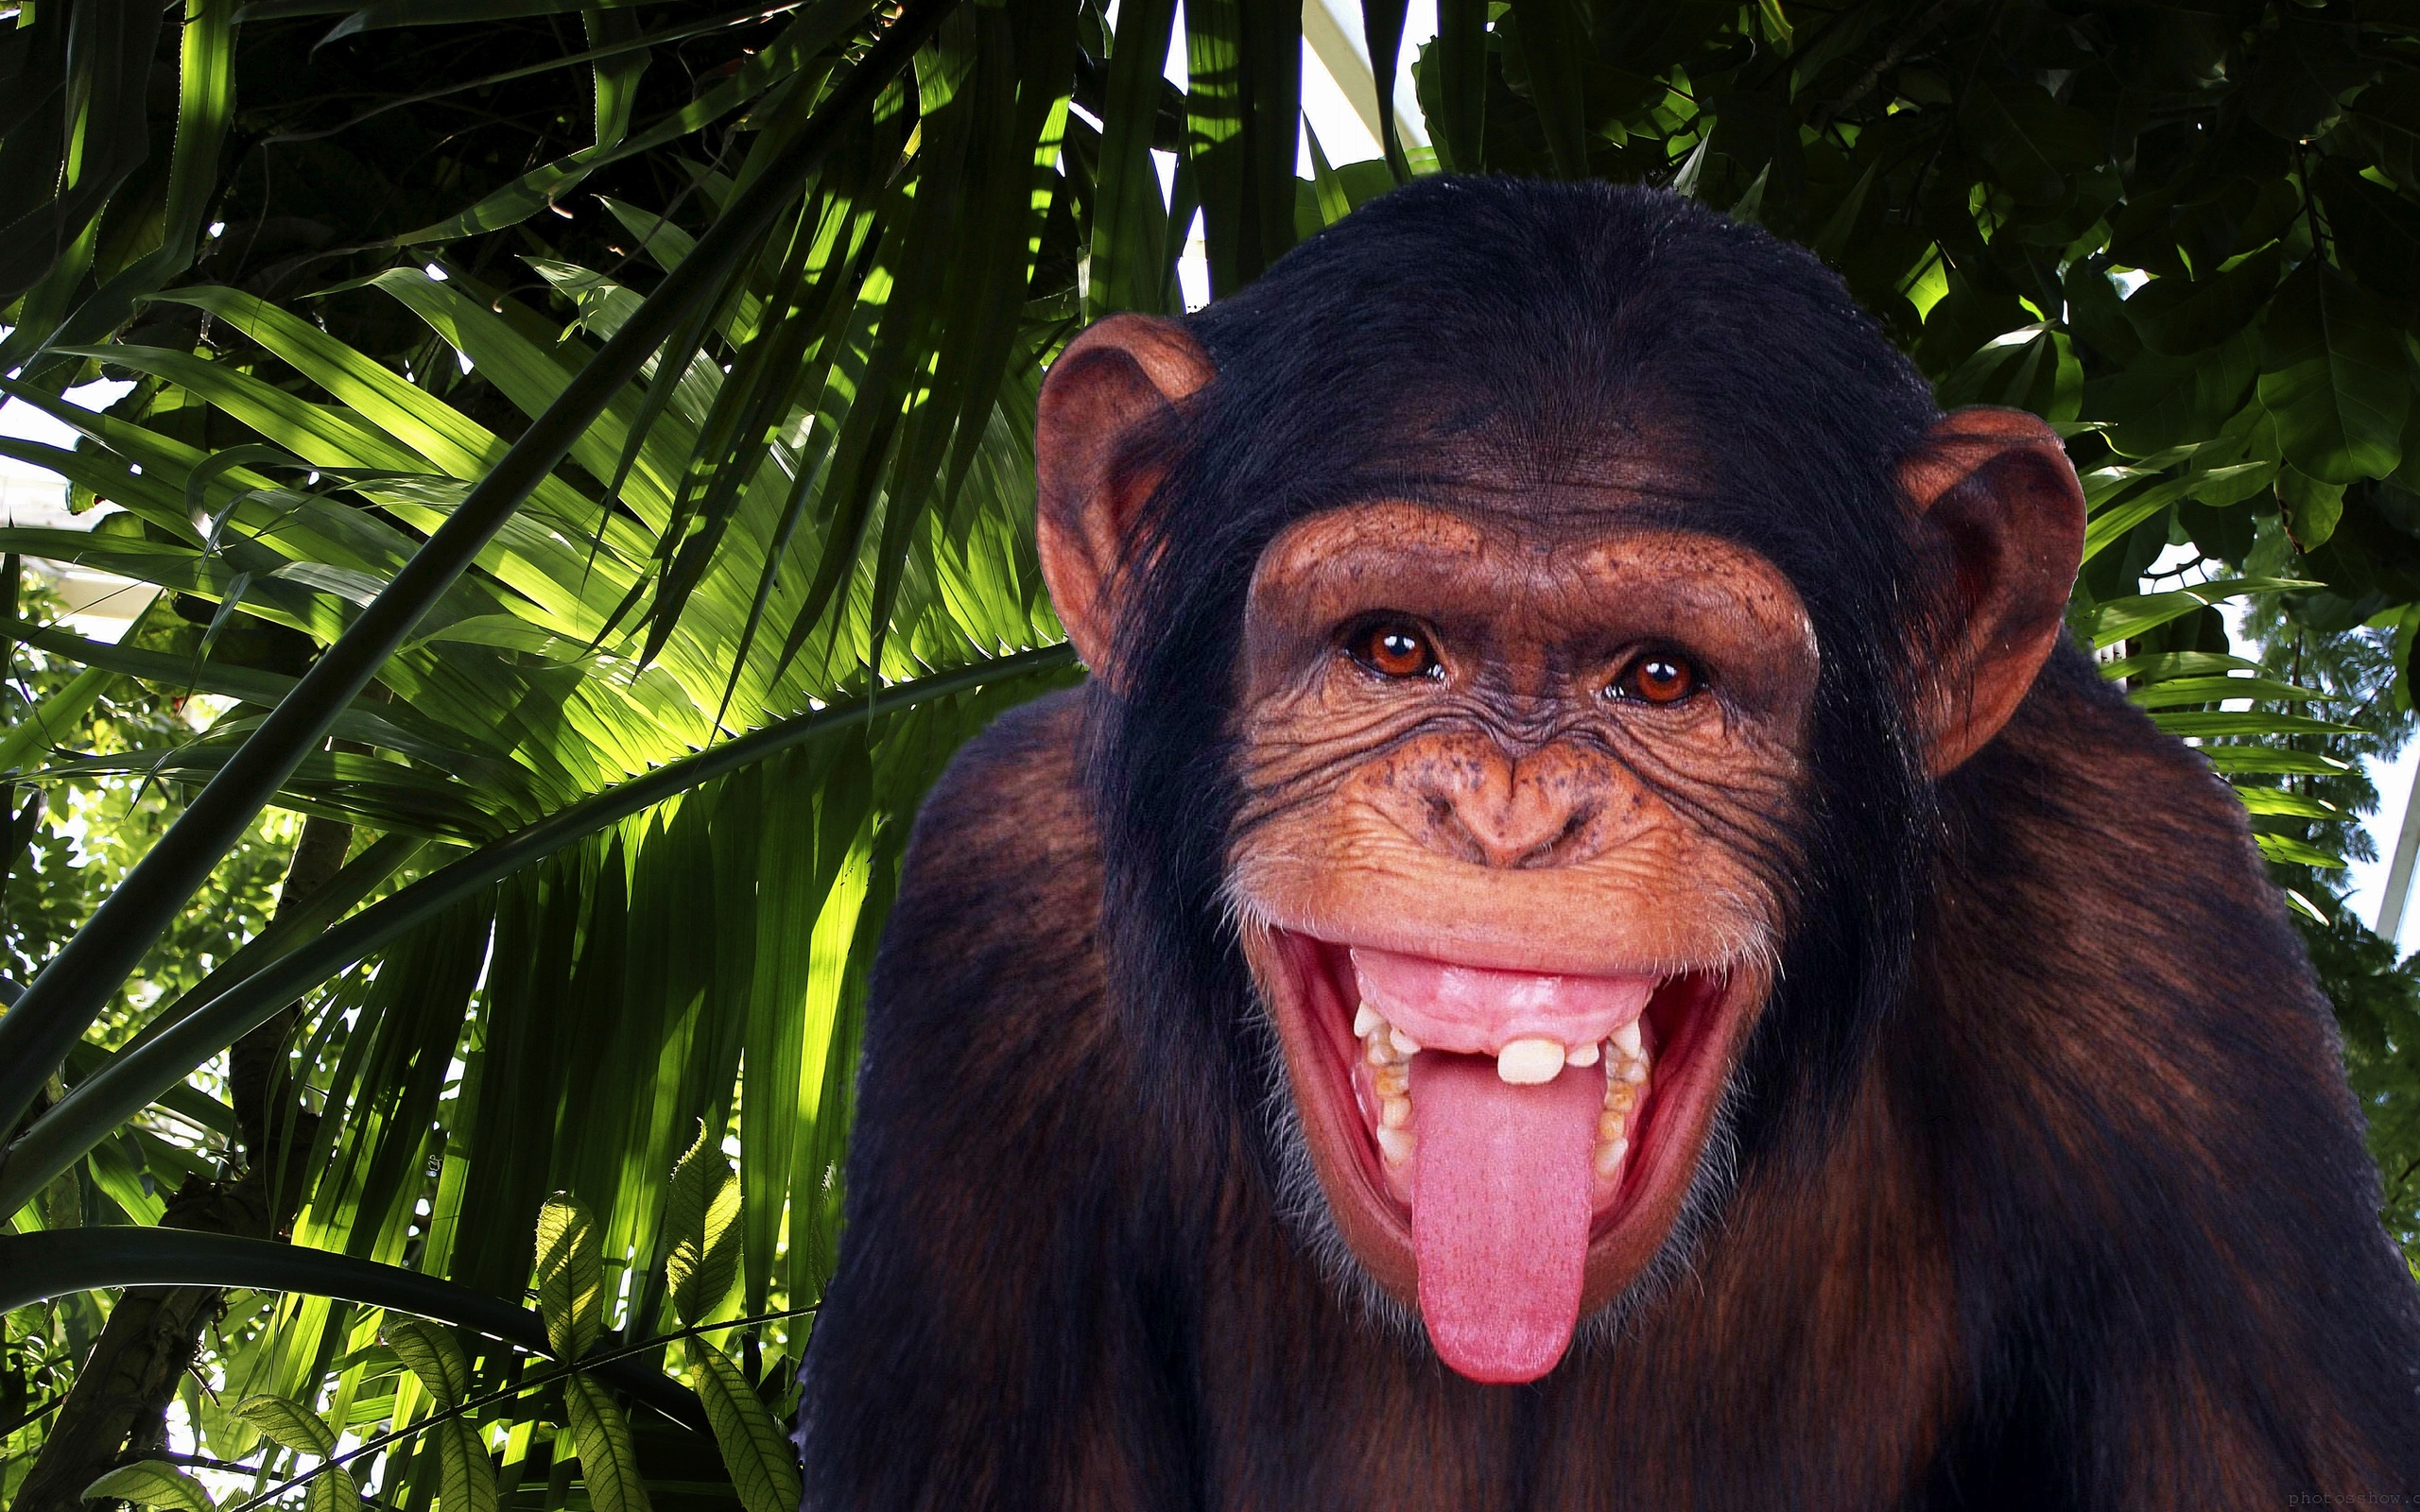
\includegraphics[scale=0.2]{monkey.jpeg}
	\section{формулы,которые должна знать каждая обезьяна}
\begin{equation}
	F = ma
\end{equation}
\begin{equation}
	S=\frac{v}{t}
\end{equation}
\begin{equation}
	a=\frac{v-v_0}{t}
\end{equation}	
\end{document}
